%!TEX root = main.tex

\section{$\tilde O(\sqrt{T})$ regret with $L$-level policy}
\label{sec:llevel}
In this section, we give an overview of how we extend our three-level
policy to a more adaptive $L$-level policy for $L > 3$ in order to
achieve a regret rate of $O_K(\sqrt{T} \polylog(T))$. We provide two
such policies. The first policy achieves the root-$T$ regret rate with
$O(\log \log T)$ levels.

% In Theorem \ref{thm:llevel-1}, we show our $L$-level policy. We can
% achieve nearly optimal regret $O_K(T^{1/2} \polylog(T))$ with
% $O(\log\log(T))$ levels.
\begin{theorem}
\label{thm:llevel-1}
For any $L > 3$, there exists an $L$-level disclosure policy with
regret $$O_K\left(T^{2^{L-1}/(2^L-1)} \cdot \polylog(T) \right).$$ In
particular, there exists a $O(\log\log(T))$-level recommendation
policy with regret $O_K(T^{1/2} \polylog(T))$.
\end{theorem}

% In Theorem \ref{thm:llevel-2}, we show a policy with
Our second policy achieves an instance-dependent regret
guarantee. This policy has the same info-graph structure as the first
one in Theorem \ref{thm:llevel-1}, but requires a higher number of
levels $L = O(\log(T/\log\log(T)))$ and larger group sizes. We will
bound its regret as a function of the gap parameter $\Delta$ even
though the construction of the policy does not depend on $\Delta$. In
particular, this regret bound outperforms the one in Theorem
\ref{thm:llevel-1} when $\Delta$ is much bigger than $T^{-1/2}$.  It
also has the desirable property that the policy does not withhold too
much information from agents---any agent $t$ observes a good fraction
of history in previous rounds.

\begin{theorem}
\label{thm:llevel-2}
There exists a $O(\log(T)/\log\log(T))$-level policy such that for
every multi-armed bandit instance with gap parameter $\Delta$, the
policy has regret $$O_K(\min(1/\Delta, T^{1/2}) \cdot \polylog(T))$$
Moreover, under this policy, each agent $t$ observes a subhistory of
size at least $\Omega( t/\polylog(T))$.
\end{theorem}

Note for constant number of arms, this result mathches the optimal
regret rate (given in \Cref{eq:model-OptRegret}) for stochastic
bandits, up to logarithmic factors.


In this section, we present the main techniques in our solution, and
the full proofs of Theorem \ref{thm:llevel-1} and Theorem
\ref{thm:llevel-2} will be deferred to Appendix
\ref{sec:llevel-details}. Similarly as Section \ref{sec:3level}, we
first prove them in the case of 2 arms (Theorem \ref{thm:llevel} and
Corollary \ref{cor:llevel}). We then extend them to the case of
constant number of arms (Theorem \ref{thm:constarm}).

A natural idea to extend the three-level policy is to insert more
levels as multiple ``check points", so the policy can incentivize the
agents to perform more adaptive exploration. However, we need to
introduce two main modifications in the info-graph two accomendate
some new challenges. We will first informally describe our techniques
for the two-arm case.

% \begin{description}
% \item[Challenge 1] \emph{Exponentially growing number of groups.} 
% \item[Challenge 2] \emph{Uncertain number of arm pulls.}  
% \end{description}


\OMIT{We will now present the main idea of extending from 3-level to
  $L$-level is that instead of using the second level as one
  ``check-point'', we use more levels to have multiple ``check
  points''.  Some new challenges appear in this process. Here we give
  an overview of the additional techniques we use to get our $L$-level
  results.}

\paragraph{Interlacing connections between levels.}A tempted approach
to generalize the three-level policy is to build an $L$-level
info-graph with the structure of a $\NG$-ary tree: for every
$l\in \{2, \ldots , L\}$, each $l$-level group observes the
sub-history from a disjoint set $\NG$ groups in level $(l-1)$. The
disjoint sub-histories observed by all the groups in level $l$ are
independent, and under the small gap regime (similar to
Lemma~\ref{3levelsmallcase}) it ensures that each arm $a$ has a
``lucky'' $l$-level group of agents that only pull $a$. This ``lucky''
property is crucial for ensuring that both arms will be explored in
level $l$.

However, in this construction, the first level will have $\NG^{L-1}$
groups, which introduces a multiplicative factor of $\NG^{\Omega(L)}$
in the regret rate. The exponential dependence in $L$ will heavily
limit the adaptivity of the policy, and prevents having the number of
levels for obtaining the result in \Cref{thm:llevel-2}. To overcome
this, we will design an info-graph structure such that the number of
groups at each level stays as $\NG^2 = \Theta(\log^2(T))$.

We will leverage the following key observation: in order to maintain
the ``lucky'' property, it suffices to have $\Theta(\log T)$ $l$-th
level groups that observe disjoint sub-histories that take place in
level $(l - 1)$. Moreover, as long as the group size in levels lower
than $(l-1)$ are substantially smaller than group size of level $l-1$,
the ``lucky'' property does not break even if different groups in
level $l$ observe overlapping sub-history from levels
$\{1, \ldots, l-2\}$.


\OMIT{In our 3-level policy, the second level has
  $\NG = \Theta(\log(T))$ groups. We do so to ensure that in the small
  gap case (Lemma \ref{3levelsmallcase}), with high probability, both
  arms are pulled enough times in the second level. The argument
  relies on the fact that agents in different second-level groups
  observe disjoint histories of the first level and the independent
  randomness in first level groups guarantees each arm $a$ to have a
  ``lucky'' second-level group such that agents in that group all pull
  arm $a$ with high probability.

  Simply generalizing this idea to an $L$-level policy would give us a
  $\NG$-ary tree like structure and the first level will have
  $\NG^{L-1}$ groups. It incurs an extra $\NG^{\Omega(L)}$ factor in
  the regret. If we use $\log\log(T)$ levels as in Theorem
  \ref{thm:llevel-1}, this factor super poly-logarithmic. If we use
  $\log(T)/\log\log(T)$ levels as in Theorem \ref{thm:llevel-2}, this
  factor goes up to polynomial in $T$.


  In order to avoid this undesirable factor, we design a slightly
  different connecting structure between levels in our $L$-level
  policy.  The key observation is that, for any level
  $l \in \{3,\ldots,L-1\}$, we do want agents in different $l$-th level
  groups to see disjoint histories of the $(l-1)$-th level to ensure
  that there is some ``lucky'' group for each arm whose mean is close
  enough to the best arm. However, it does not matter much if pulls in
  levels below $l-1$ get observed by agents in different $l$-th level
  groups because group sizes in lower levels are much smaller than
  group sizes of level $l-1$ and the independent randomness in level
  $l-1$ is sufficient.}

This motivates the following interlacing connection structure between
levels. For each level in the info-graph, there are $\NG^2$ groups for
some $\NG = \Theta(\log(T))$. The groups in the $l$-th level are
labeled as $G_{l,u,v}$ for $u,v\in[\NG]$. For any $l \in \{2,\ldots,L\}$
and $u,v,w\in [\NG]$, agents in group $G_{l,u,v}$ see the history of
agents in group $G_{l-1,v,w}$ (and by transitivity all agents in
levels below $l-1$). See Figure \ref{fig:llevel-connecting} for a
visualization of simple case with $\NG = 2$). Two observations are
in order:
% \OMIT{(i) The number of groups does not grow with $L$ and stays as
%   $\NG^2 = \Theta(\log^2(T))$ in each level. Having these groups only
%   incurs a $\Theta(\log^2(T))$ multiplicative factor to the regret.\\}
\begin{itemize}
\item[(i)] Consider level $(l - 1)$ and fix the last group index to be
  $v$, and consider the set of groups
  $\cG_{l-1, v}=\{G_{l-1,i,v}\mid i \in [\NG]\}$ (e.g. $G_{l-1,1,1}$
  and $G_{l-1,2,1}$ circled in red in the Figure
  \ref{fig:llevel-connecting}). The agents in any group of
  $\cG_{l-1, v}$ observe the same sub-history. As a result, if the
  empirical mean of arm $a$ is sufficiently high in their shared
  sub-history, then all groups in $\cG_{l-1, v}$ will become ``lucky''
  for $a$.

\item[(ii)] Every agent in level $l$ observes the sub-history from
  $\NG$ $(l-1)$-th level groups, each of which belonging to a
  different set $\cG_{l-1, v}$. Thus, for each arm $a$, we just need
  one set of groups $\cG_{l-1, v}$ in level $l-1$ to be ``lucky'' for
  $a$ and then all agents in level $l$ will see sufficient arm $a$
  pulls.
 \OMIT{For each set of groups
    in level $l-1$, agents in level $l$ see the history of agents in
    one of these groups. Therefore, for each arm $a$, we just need one
    set of groups in level $l-1$ to get ``lucky'' and then all agents
    in level $l$ will see enough pulls of arm $a$.}
\end{itemize}

\begin{figure}[H]
\centering
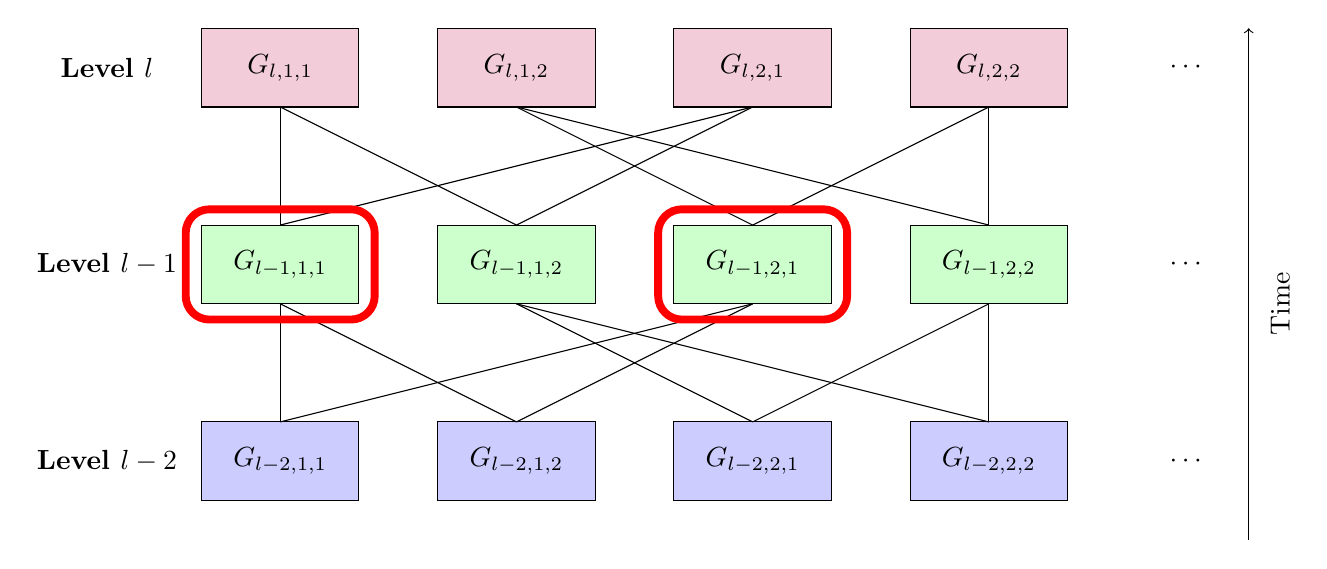
\begin{tikzpicture}  
 \foreach \x in {0,3,6,9}
 {
 \filldraw[fill=purple!20!white]
 (\x+0,7.5)--(\x+2,7.5)--(\x+2,8.5)--(\x+0,8.5)--cycle;
 \filldraw[fill=green!20!white]
 (\x+0,5)--(\x+2,5)--(\x+2,6)--(\x+0,6)--cycle;
 \filldraw[fill=blue!20!white]
 (\x+0,2.5)--(\x+2,2.5)--(\x+2,3.5)--(\x+0,3.5)--cycle;
 }
\foreach \y in {2.5,5,7.5}
{
  \node at (12.5,\y+0.5){$\cdots$};
} 


\foreach \y in {3.5,6}
{
  \draw (1,\y) -- (1,\y+1.5);
  \draw (1,\y) -- (7,\y+1.5);
  
  \draw (4,\y) -- (1,\y+1.5);
  \draw (4,\y) -- (7,\y+1.5);
  
  
  \draw (7,\y) -- (4,\y+1.5);
  \draw (7,\y) -- (10,\y+1.5);
  
  
  \draw (10,\y) -- (4,\y+1.5);
  \draw (10,\y) -- (10,\y+1.5);
} 

\foreach \u in {1,2}
{
	\foreach \v in {1,2}
	{
	\pgfmathsetmacro{\x}{((\u-1)*2+(\v-1))*3};
	\pgfmathsetmacro{\xa}{((\u-1))*3};
	\pgfmathsetmacro{\xb}{(2+(\u-1))*3};
   \node at(\x+1,8){$G_{l,\u,\v}$};
   \node at(\x+1,5.5){$G_{l-1,\u,\v}$};
   \node at(\x+1,3){$G_{l-2,\u,\v}$};
	}
}


  \node at(-1.2,3){\textbf{Level $l-2$}};
  \node at(-1.2,5.5){\textbf{Level $l-1$}};
  \node at(-1.2,8){\textbf{Level $l$}};
  \draw[->] (13.3,2)--(13.3,8.5);
  \node at(13.7,5)[ rotate=90]{Time};

 \draw [rounded corners=3mm, line width=1mm, red](-0.2,4.8)--(2.2,4.8)--(2.2,6.2)--(-0.2,6.2)--cycle;
  \draw [rounded corners=3mm, line width=1mm, red](5.8,4.8)--(8.2,4.8)--(8.2,6.2)--(5.8,6.2)--cycle;
\end{tikzpicture}
\caption{Connecting structures between levels for the $L$-level policy.}
\label{fig:llevel-connecting}
\end{figure}

\paragraph{Amplifying groups for boundary cases.} Recall in the
three-level policy, the medium gap case (Lemma \ref{3levelmedium})
corresponds to the case where the gap $\Delta$ is between
$\Omega\left({{1}/{T_1}}\right)$ and
$O\left(\sqrt{{\log(T)}/{T_1}}\right)$. This is a boundary case since
$\Delta$ is neither large enough to conclude that with high
probability agents in both the second level and the third level all
pull the best arm, nor small enough to conclude that both arms are
explored enough times in the second level (due to
anti-concentration). In this case, we need to ensure that agents in
the third level can eliminate the inferior arm. This issue is easily
resolved in the three-level policy since the agents in the third level
observe the history of the entire first level, which provides
sufficiently accurate reward estimates for both arms.

\OMIT{about the situation in which the sub-optimal arm does not get
  pulled enough times in the first two levels and some agents in the
  third level may pull the sub-optimal arm.  Such situation is
  naturally ruled out in our 3-level policy for the following
  reason. Agents in the third level observe the history of the entire
  first level while agents in the second level only observes the
  history of a single first-level group. For each arm, even if it is
  not explored enough times in the second level, its empirical mean
  concentrates closer to its actual mean in the history observed by a
  third-level agent than the one observed by a second-level
  agent. Therefore, although the gap in the medium gap case is just
  not large enough for agents in the second level to all pull the best
  arm, it is large enough for agents in the third level to all pull
  the best arm.}

When we extend the 3-level policy to an $L$-level policy, we have such boundary case for each intermediate level. Moreover, the worry mentioned above does not get naturally resolved as in some of these boundary cases, the ratios between the upper and lower bounds of the gap rise from $\Theta(\sqrt{\log(T)})$ to $\Theta(\log(T))$. The reason for such rise is that, except the first level, we don't have good enough guarantee of the number of pulls of each arm. For example, in Figure \ref{fig:llevel-connecting}, when we talk about having enough arm $a$ pulls in the history observed by agents in $G_{l,1,1}$, it could be that  only agents in group $G_{l-1,1,1}$ are pulling arm $a$ and it also could be that most agents in groups $G_{l-1,1,1},G_{l-1,1,2},...,G_{l-1,1,\NG}$ are pulling arm $a$. Therefore our estimate of the number of arm $a$ pulls can be off by an $\NG=\Theta(\log(T))$ multiplicative factor. This finally makes the boundary cases harder to deal with.

In our $L$-level policy, after understanding the boundary cases well, we resolve this problem by introducing an additional type of groups: $\Gamma$-groups. For each $l \in [L], u,v \in [\NG]$, we create a $\Gamma$-group $\Gamma_{l,u,v}$. Agents in $\Gamma_{l,u,v}$ observe the same history as the one observed by agents in $G_{l,u,v}$ and the number of agents in $\Gamma_{l,u,v}$ is $\Theta(\log(T)$ times the number of agents in $G_{l,u,v}$. The main difference between the $G$-groups and $\Gamma$-groups is that the history of $\Gamma$-groups in level $l$ is not sent to agents in level $l+1$ but agents in higher levels. When we are in the boundary case in which we don't have good guarantees about the $l+1$ level agents' pulls, the new construction makes sure that agents in levels higher than $l+1$ get enough pulls of each arm and all pull the best arm. 
%%% Local Variables:
%%% mode: latex
%%% TeX-master: "main"
%%% End:
